\documentclass{article}
\usepackage{geometry}
 \geometry{
 a4paper,
 total={170mm,257mm},
 left=20mm,
 top=20mm,
 }
\usepackage[utf8]{inputenc}
\usepackage[T1]{fontenc}
\usepackage[english]{babel}
\usepackage[language=english, style=numeric, sorting=none]{biblatex}
\usepackage{lipsum}
\usepackage{hyperref}
\hypersetup{
    colorlinks=true,
    linkcolor=blue,
    filecolor=magenta,      
    urlcolor=blue,
}


\newcommand{\lecture}[2]{
  \pagestyle{myheadings}
  \thispagestyle{plain}
  \newpage
%   \setcounter{lecnum}{#1}
  \setcounter{page}{1}
   \noindent
   \begin{center}
   \framebox{
      \vbox{\vspace{2mm}
    \hbox to 6.28in { {\bf ELP 305: Design and Systems Laboratory
        \hfill Semester II 2020-2021} }
       \vspace{4mm}
       \hbox to 6.28in { {\Large \hfill Laboratory Report, Group H: #2  \hfill} }
       \vspace{2mm}
       %\hbox to 6.28in { {\it Course Coordinator: Prof. Subrat Kar \hfill} }
      \vspace{2mm}}
   }
   \end{center}
   % Write your entry numbers here
    %\vspace{2mm}\\
    \noindent
    \noindent
    {\bf Note}: {\it LaTeX template courtesy of UC Berkeley EECS dept. %% \cite{noauthor_latex_nodate}
    }
    
   \vspace*{10mm}
}

% ADD YOUR PACKAGES HERE
\usepackage{amsmath,amsfonts,graphicx,courier,listings,float}
\newcommand{\eat}[1]{} %% for block comments

%% For TOC
\usepackage{titletoc}
\usepackage[toctitles]{titlesec}

%% for codes
% \usepackage[boxruled,linesnumbered]{algorithm2e} % Algo formatting
\usepackage{listings}
\usepackage{color}
\definecolor{mygreen}{rgb}{0,0.6,0}
\definecolor{mygray}{rgb}{0.5,0.5,0.5}
\definecolor{mymauve}{rgb}{0.58,0,0.82}
\definecolor{mybg}{rgb}{0.98,0.98,0.98}

\lstset{ %
  backgroundcolor=\color{mybg},          % choose the background color
  basicstyle=\ttfamily\footnotesize,     % size of fonts used for the code
  commentstyle=\color{mygreen},         % comment style
  % escapeinside={\%*}{*)},             % if you want to add LaTeX within your code
  keywordstyle=\color{blue},            % keyword style
  captionpos=b,                         % sets the caption-position to bottom
  stringstyle=\color{mymauve},     % string literal style
  tabsize=4,                       % tab size
  breaklines=true,                 % automatic line breaking only at whitespace
  keepspaces=true,                  % for proper indendations at the beginning in python
  numbers=left,                     % display line numbers
  numberstyle=\tiny\color{mygray},
  numbersep=7pt,
  breakatwhitespace=false,
}

% \usepackage{pdfpages} % attach pdf

% ADD YOUR REFERENCES IN THIS FILE
\addbibresource{ref.bib} 

\newtheorem{theorem}{Theorem}
\newtheorem{proposition}{Proposition}

\begin{document}
\lecture{1}{Mule Bot-Communication}

\begin{tabular}{ |p{0.7cm}|p{5cm}|p{3.1cm}|p{6cm}|  }
 \hline
 \multicolumn{4}{|c|}{\textbf{\textit{Members of the group H}}} \\
 \hline
 \hline
 Sl & \textbf{Position} & \textbf{Entry Number} & \textbf{Name}\\
 \hline
 \hline
1 & \textbf{Lead Coordinator} & 2018EE10593 & Arunava Das \\ \hline
2 & Hardware Coordinator & 2018EE10603 & Dedeepyo Ray \\ \hline
3 & Hardware Sub-Coordinator & 2018EE30569 & Yerukula Sravanasai \\ \hline
4 & Software Coordinator & 2018MT60798 & Zuhaib ul Zamann \\ \hline 
5 & Documentation Coordinator & 2018MT10770 & Subhalingam D \\ \hline
6 & Doc Sub-Coordinator & 2018MT10759 & M Santosh \\ \hline
7 & Member(B) & 2018MT60795 & Snehil Grandhi \\ \hline
8 & Member(A) & 2018EE10459 & Chathur Gudesa \\ \hline
9 & Member(B) & 2018EE30610 & Harsh Wardhan \\ \hline
10 & Member(D) & 2018MT10756 & Ishant Bhaskar \\ \hline
11 & Member(B) & 2018MT60787 & Prateek Singh \\ \hline
12 & Member(D) & 2018EE30538 & Dharmendra Seervi \\ \hline
13 & Member(D) & 2018EE30543 & Himanshu Gaud \\ \hline
14 & Member(A) & 2018MT60793 & Satendra Singhparashar \\ \hline
15 & Member(A) & 2018EE10494 & Rohit Agarwal \\ \hline
16 & Member(D) & 2018MT10737 & Akshat Rao \\ \hline
17 & Member(A) & 2018MT60790 & Ravi Pushkar \\ \hline
18 & Member(B) & 2018MT60788 & Ramneek Singhgambhir \\ \hline
19 & Member(D) & 2018MT60776 & Aakash Garg \\ \hline
20 & Member(D) & 2018EE30534 & Darpan Kumaryadav \\ \hline
21 & Member(A) & 2018EE10499 & Shashank Goyal \\ \hline
22 & Member(B) & 2018MT60786 & Pranaav \\ \hline
23 & Member(B) & 2018MT60779 & Bhupender Dhaka \\ \hline
24 & Member(B) & 2018EE10491 & Ranajay Medya \\ \hline
25 & Member(B) & 2018EE10189 & Aditya Bansal \\ \hline
26 & Member(A) & 2018MT60777 & Adwaith H Sivam \\ \hline
27 & Member(B) & 2018MT60791 & Rishu Raj \\ \hline
28 & Member(B) & 2018EE10483 & Penumudinagavenkata Saiabhinay \\ \hline
29 & Member(A) & 2018MT10740 & Anirudha Akela \\ \hline
30 & Member(B) & 2018EE30598 & Bharat Runwal \\ \hline
31 & Member(A) & 2018EE30558 & Reddy Cihir \\ \hline
32 & Member(A)	& 2018MT60778 &	Ashwini Kumar \\ \hline
33 & Member(D)	& 2018MT10745 & Aryan Gupta \\ \hline
34 & Member(B)	& 2018MT60244 & Shaurya Goyal \\ \hline
35 & Member(B)	& 2018MT10763 & Punit Shyamsukha \\ \hline
36 & Member	& 2018MT10760 & Mukul Kumar \\ \hline
37 & Member	& 2018MT60797 & Vishal Meena \\ \hline
38 & Member	& 2018EE10514 & Vikas Kumar \\ \hline
39 & Member(A)	& 2018MT60199 & Anshul Tak \\ \hline
40 & Member(A)	& 2018EE10456 & Biruduraju Harahima dhruthi  \\ \hline
\end{tabular}
\newpage
 \tableofcontents
\newpage

\section{Introduction}
The Mule Bot proposed in our previous report\footnote{Report available at  \url{https://owncloud.iitd.ac.in/nextcloud/index.php/s/Dq33TD69n69fF7c} \textit{(Section 4.5)}} can be reformed to include communication\eat{( As said in Sec 4.5 Point 6)}. For this, first a protocol needs to be defined, based on which we can then specify the specifications of the technology to be used and the protocols it would follow.

\section{Network Architecture}

Bots connect to antennas (i.e., wireless routers/repeaters/wireless access points). These are connected to a central server. If the mall is large, then each floor can have its own hub where the antennas connect to, and then these hubs can be connected to the central server.
\\ \\
The information in the server can be stored in a \textbf{SQL database} as the data will be of fixed format. The \textbf{attributes} to be stored includes \textit{charge level}, \textit{location}, \textit{current status} (idle or in-use), etc. More attributes can be added depending on the features desired. The data in these attributes would be updated periodically to the server by the bot. Moreover we can also store some statistical data such as weight carried around by the bot, total distance travelled in a day, number of customers served and so on. Such additional information would be useful in analysing and studying potential areas of improvements in the future. \eat{These data then can be analysed for detecting potential areas of improvement in future.}
\\ \\
We can have an open port on the central hubs and server which will listen for distress signals sent by the bots in case of accident or malfunction.

\begin{figure}[h]
    \centering
    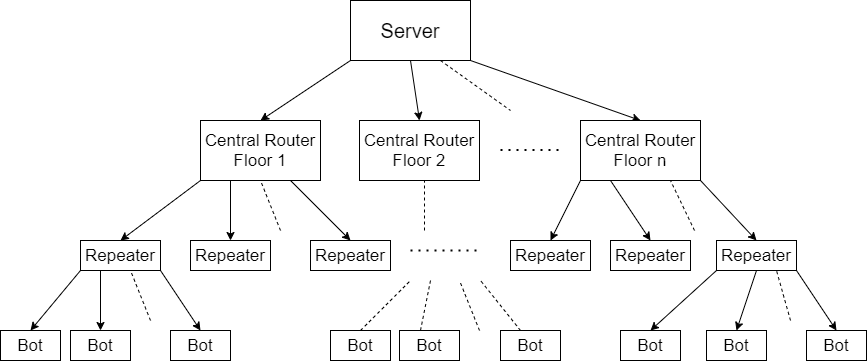
\includegraphics[scale=0.5]{Images/Communication.png}
    \caption{Architecture of the Network}
\end{figure}

\section{Choosing the Communication Technology}
\subsection{Discarded Technologies}
The technologies which we have discarded are listed below, each with the reason as to why they do not fit in our model of Mule Bot communication:
\begin{enumerate}
    \item \textbf{BLE:} Not ideal as the range is too small.
    \item \textbf{Radio:} Old technology, and can cause radio interference causing miscommunication.
    \item \textbf{Infrared:} High unreliability and would need extra hardware on RPi.
    \item \textbf{ESP32:} Too long range, and high cost factor. Essentially similar to WiFi but with more intensive hardware requirements. \cite{ESP32}
\end{enumerate}
Eliminating these, we now have quite a few choices for the technology specifications of communication. First we explore the two front-runners in our case in the following two subsections.
\subsection{2.4GHz Technology}
\begin{itemize}
\item \textbf{Wi-Fi standard IEEE 802.11b operating frequency}.
\item It provides \textbf{slower data frequency} (slower than 5 GHz).
\item It has a \textbf{good range} (410 feet practically).
\item It has a \textbf{bandwidth lower than 5 GHz frequency}.
\item It is used for surfing at distances, stream for basic needs.
\item It reaches \textbf{150 feet indoors} and \textbf{300 feet outdoors}.
\item It is \textbf{great for public use}. For example, it is used in libraries, cafeteria, etc.
\item \textbf{RPi has inbuilt WiFi} - so no extra cost is incurred. We can build a home server using an RPi.
\item \textbf{Daisy chaining in WiFi} can be done easily.
\end{itemize}

\subsection{5GHz Technology}
\begin{enumerate}
\item \textbf{Wi-Fi standard IEEE 802.11a operating frequency}.
\item It provides \textbf{fast data frequency}.
\item It is good to use for \textbf{short distances}.
\item It has \textbf{bandwidth higher than 2.4 GHz frequency}.
\item It is useful for streaming long videos and downloading.
\item It reaches \textbf{50 feet indoors} and \textbf{100 feet outdoors}.
\item It is mostly used for \textbf{personal and business use}.
\end{enumerate}

\subsection{Advantages of using 2.4GHz over 5GHz for Mule-Bot Communication}
The main reasons why 2.4GHz technology stands out for our purpose is summarised in the following points:
\begin{enumerate}
\item A 2.4GHz connection travels farther at lower speeds, while 5GHz frequencies provide faster speeds at shorter range. As \textbf{communication between Mule Bots is not restricted to short range}, \textbf{2.4GHz is ideal} for our purpose.
\item \textbf{2.4GHz is better at penetrating solid objects} than 5GHz. \cite{WiFi_comparison} So, Mule Bots can easily communicate from one room to another in the former. They can also communicate if there is solid material type obstacles.
\item 2.4GHz is \textbf{cheaper} than 5GHz.
\item 2.4GHz uses \textbf{less power} in comparison to 5GHz.
\end{enumerate}

\subsection{Setting up the WiFi}
The 2.4GHz WiFi communication system can be easily set up with the already available Raspberry-Pi unit we had in our Mule Bot, without much extra hassle \cite{Setting_up_wifi}. We will need access to the Pi’s command prompt. We just need to type the following command line to initiate the connection \cite{wifi_rpi3}:
\begin{lstlisting}[language=Bash]
sudo iwlist wlan0 scan
\end{lstlisting}
The Raspberry Pi comes with an on-board 802.11n Wireless LAN adapter, but this has a short detection range so we use a separate transceiver \cite{transceiver} alongside the setup to enhance inter-bot communication.
\newpage
\section{Antenna Topology}
We will use a circular topology for our wireless sensor/router network.
The advantages of circular topology is its \textbf{ease-of-maintenance}, \textbf{ease-of-use} and \textbf{efficiency}.
\\ \\
An approximate center of the roof of the mall is found, and we place a ``sink'' router at this position. Concentric circles are drawn around
this sink and on the circumference of each circle, we place the required
number of routers (which will be proportional to the circumference of
that circle). The radii of the concentric circles and the number of
routers per circle are chosen such that every point falls within the
range of at least one sensor. However, the geometry is chosen such that
no point is covered by more than 3 routers.

\begin{figure}[htp]
    \centering
    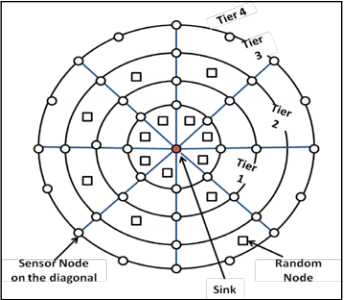
\includegraphics[scale=0.9]{Images/t1.png}
    \caption{Circular Topology \cite{antenna}}
    \label{fig:galaxy}
\end{figure}

\noindent For the Mule Bot to send and receive data, it first picks up the signal of
any router that covers that position (if multiple routers cover that
position, any one is selected at random). Then the mule bot sends
information to this router, which in turn passes it to the closest router
on the concentric circle one tier less than it, and
this in turn is repeated until the information arrives at the sink. The
sink, using a similar process, sends the information to the receiving
Mule Bot.
\\ \\
It is assumed that the sink keeps track of the approximate location of the mule bots, so it knows where to send the information received. This is achieved by having the active mule bots send their current location to the sink every 10 seconds and storing it.

\subsection{How many Routers do we need?}

The number of routers we would require if we were to use this topology would depend on the size of the mall and the range of the routers. The routers we are using have a range of a maximum range of $410ft$ but we will assume a range of $300ft$ because obstacles might decrease the strength of the signal. If we consider an average superior grade mall size of 4,00,000 square feet, then we would require around $\approx\ 2 \times \frac{4,00,000}{300 \times 300}\ =\ 9$ routers. 
\\ \\
If we assume the roof of the mall to be square-shaped, then the length of it would be around $650ft$. In such a case, we place the sink router at the center of the square and distribute the remaining routers along the circumference of two concentric circles with radii $150ft$ and $400ft$ respectively. On each of these concentric circles we place 4 routers each separated by $90^{\circ}$.
\\ \\
In summary, we will require a total of $9$ routers/antennae for an average superior grade-sized mall.

\section{Transceiver}
\textbf{\emph{NRF24L01 2.4GHz Wireless Transceiver Module}}
\begin{figure}[h]
    \centering
    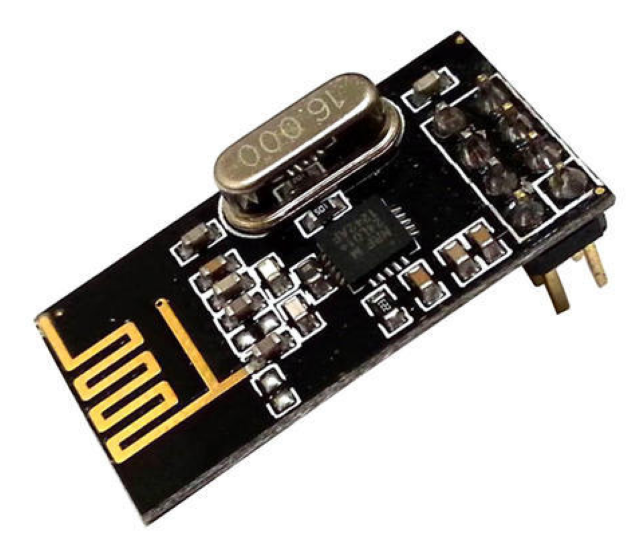
\includegraphics[scale=0.5]{Images/Transceiver.png}
    \caption{Transceiver Module}
    \label{fig:my_label}
\end{figure}

\begin{center}
       \begin{tabular}{|l|l|}
            \hline
            Band & 2.4-2.5 GHz\\
            \hline
            Max Operating Speed & 2Mbps\\
            \hline
            Communication range & 40 to 100m\\
            \hline
            Compatability & Arduino and Raspberry Pi\\
            \hline
             L$\times$W$\times$H(mm) & 20$\times$15$\times$13\\
            \hline
            Weight & 8g\\
            \hline
            \end{tabular}
            \end{center}
\textbf{2.4GHz Transmitter and Receiver NRF24L01 Module Board}
\\
This transceiver consists of fully integrated frequency synthesizer,na power amplifier, a crystal oscillator, a demodulator, modulator and enhanced shock burst protocol engine. It has anti-interference ability, built-in antenna and CRC errors detection with less current consumption, which is good for transferring data.

\section{Basic Communication Protocols}
First we address the basic communication protocols that these Mule Buts and the network must have for a smooth functioning. We can break down the essential protocols into three sub-groups and address each in an algorithmic way:
\subsection{Charging of the Mule-Bot}
\begin{enumerate}
    \item If charge is low (~15\%) for a bot already in use, we need to call a fully charged bot from the charging platform to the user and return the current bot to the charging platform. Also, an alarm can be sent to the user app indicating low signal and the approximate time remaining for replacement.
    \item If the charging requirement of multiple bots exceeds the number of currently available charging points, priority needs to be assigned accordingly based on the distance of bots from the charging platform. A possible algorithm is given below:
    \begin{itemize}
        \item The first order assigned to the bots closest to each platform within a radius of $R_1$.
        \item Then assign bots between radius $R_1$ to $R_2$ for the platforms with vacancy.
        \item Then assign bots between radius $R_2$ to $R_3$ for the platforms with vacancy.
        \item If platform is at capacity at any iteration, stop intake of bots for that platform.
        \item After all the platforms have been assigned to $R_3$, if $n$ number of bots are left, there will be $n$ empty slots in different platforms. Then we can assign bots to platforms according to the bot serial numbers (stored in the central server SQL database).
    \end{itemize}
\end{enumerate}
\subsection{Path selection of the Mule-Bots}
\begin{enumerate}
    \item If there is another bot within $r$ radius of a bot, and the bot that has been detected as well as the detector bot are travelling to the same station, they may follow a line to avoid collisions.
    \item Similar protocols can also be used if some people (e.g., family) want to shop together. We can include functions like merge bots before the family goes to the payment queue.
\end{enumerate}
\subsection{Malfunction of Mule-Bot}
If a mule bot starts behaving abnormally, i.e., it breaks down due to some issue (circuit issue, overloaded, battery problem, etc.) requiring immediate human intervention, it should send a signal back to the central server, which will be relayed to the service team requesting for help. It must also send a mule bot immediately for replacement.
%%%%%%%%%%%%%%%%%%%%%%%%%%%%%%%%%%%%%%%%%%%%%%%%%%%%%%%%%%%%%%%%%%%%%%

\section{Detailed Communication Protocols}
Here we present the detailed description of the protocols that these bots have between themselves. Each subsection has a description followed by a hyperlink to the related code description in Appendix \ref{appendix:code}.
\subsection{ Protocol for efficient charging of bots}
\textbf{Task: } If a bot is 100\% charged and is currently on charge, it will yield the charging point for other bots. \\ \\
The source code can be found in \ref{code:a}.

\subsection{Replacement of malfunctioning Bot}
\textbf{Task: } If a bot crashes or has low battery, communication protocol can be used to allow a nearby free bot with sufficient energy levels to replace itself with the crashed  bot, giving customer information about the exchange at the same time. If no nearby bot is available, we can request a bot from the main docking/charging station to replace this bot. Then, while the other bot is deployed or is on the way, the current bot can go into low power mode where it would slowly follow the customer while the other bot arrives. It keeps checking if the deployed bot is near and is available and free, then it would turn off and proceed to give control to the other bot (change the variable of being used or not).
\\
\\
The source code can be found in \ref{code:b}.

\subsection{Heavy baggage case}
\textbf{Task: } For customers with baggage needs of more than $40kg$, communication protocol can be used to bring a new bot that can be merged with the current bot (one bot will follow other) and satisfy the requirement.
\\
\\
The source code can be found in \ref{code:c}.
\subsection{Unexpected Shutdown}
\textbf{Task: } After a while, the low powered bot would try to find its way back to the charging dock. However, it may be possible that the low powered bot cannot find its way to the station. In that case, it would shut down and manual assistance would be required to take it back.
\\
\\
The source code can be found in \ref{code:d}.
\subsection{Loading-Unloading of materials in mall}
\textbf{Task: } Special tasks like loading material from the basement to a room in the mall using bots can be done using the communication protocol. Bots with material going in the same rule will follow on after the other and unloading will be done in the room (like \textit{worker ants}).
\\
\\
The source code can be found in \ref{code:e}.
\subsection{Checking Bot performance and health}
\textbf{Task: } Bot performance and health can also be checked using communication protocol.
\\
\\
The source code can be found in \ref{code:f}.
\subsection{Clearing left over items}
\textbf{Task: } Some customers might leave some materials which they initially thought of buying but lost interest later on. This can be redirected to a docking station where there is a clearance.
\\
\\
The source code can be found in \ref{code:g}.
\subsection{Reducing bot traffic in congested areas}
\textbf{Task: } If more than $m$ bots are present in a radius of $R$, it will generate a signal and unused bots will be redirected to other places where there are less number of bots to avoid congestion. This will happen only during working hours.
\\
\\
The source code can be found in \ref{code:h}.
\subsection{Avoiding bot collisions}
\textbf{Task: } If there are two bots, one bot with a user and the other bot is within $2m$ of its position, a signal should be transmitted so that these bots can be kept informed about presence of each other to avoid collisions.
\\
\\
The source code can be found in \ref{code:i}.
\subsection{Deployment of reserve bots for better user experience}
\textbf{Task: } If the number of working bots drops below a threshold, the communication protocol can be used to deploy reserve bots to fill the gap and the security will be alerted.
\\
\\
The source code can be found in \ref{code:j}.
\subsection{Customized baskets for varied purchases}
\textbf{Task: } Sometimes customers need different baskets for different purchases. Communication protocol can be used to allot those bots to the customer which have the requested basket attached to them (if any such bot is already free).
\\
\\
The source code can be found in \ref{code:k}.
\subsection{Avoiding redundancies in group purchases}
\textbf{Task: } If a family/group has come to a mall, the corresponding bots assigned to the family/group members can be put in communication with each other to let family/group members know of each other's purchases and inform them of multiple purchases of the same item by different members of the family.
\\
\\
The source code can be found in \ref{code:l}.
\subsection{Conserving battery/Sentry mode}
\textbf{Task: } Communication protocol can be used to put the Bot in \textbf{standby mode} (in secure mode, no item can be pulled out/put in) when the customer is in the lavatory. The bots will wait for the customer in a specified waiting area specified by the mall close to the lavatory to avoid clustering in the lavatory.
\\
\\
The source code can be found in \ref{code:m}.
%%%%%%%%%%%%%%%%%%%%%%%%%%%%%%%%%%%%%%%%%%%%%%%%%%%%%%%%%%%%%%%%%%%%%%
\section{Handling race conditions}
Various responses by the bots have been automated using communication protocols. Cases may arise when a bot will have a state that leads to two or more than two of those automated responses. In those cases, we specify the priority of responses which the bot will follow if the need arises.
\begin{enumerate}
    \item The total number of workable bots in the mall is below threshold (Priority = 0).
    \item A bot calls for manual assistance in case of unexpected Shutdown (Priority = 1).
    \item A bot in case of low battery condition calls for another bot for replacement (Priority = 2).
    \item  Bot enters a congested area and initiates clearing protocol (Priority = 3).
    \item In case of heavy baggage bot stops moving and asks the user to either reduce the baggage weight or call an extra bot (Priority = 4).
    \item Free bot is called for loading/unloading of materials in the mall (Priority = 5).
\end{enumerate}
If two or more of these situations arise, then the situation with lowest priority value will be the bots first response.
If this response of the bot does not address all the situations, then the next uncleared situation with lowest priority value will be dealt by the bot. This process continues till all the issues are resolved.
%%%%%%%%%%%%%%%%%%%%%%%%%%%%%%%%%%%%%%%%%%%%%%%%%%%%%%%%%%%%%%%%%%%%%%
\section{Specifications of Charging stations and storing Mule-Bots}
We consider a general layout of mall. Specifications will change as the mall layout changes. Consider a mall with $M$ floors, with base of dimensions 
$L \times B$. Let the average maximum number of customers that are present in the mall at a time during working hours on a floor be $A$. We recommend assigning $2A$ bots to each floor and keeping $A$ bots as reserve bots.\\ \\
A good working condition for the bots is when $L\times B \geq 32\times A\times \text{area}(Bot)$\\
\begin{enumerate}
    \item Each floor will have $4$ charging stations which are placed on four corners of the rectangle, which the base of the floor makes.
    \item Each charging station should have space enough to charge at least $A/2$ bots. Bots will be stored only in the basement of mall.
    \item A bot will be stored if it is broken or is an emergency (reserve bot) only. All other bots be kept inside the charging station when the working hours of the mall are over.
    \item A charging station will have proper guides that will serve as paths for bots to follow so that the alignment of the bots saves space.
    \item Each guide path will have an adjacent leaving path which will allow any bot (in the middle or front or back of the line) to be able to leave without disturbing other bots.
    \item  Charging bots will readjust their charging spaces once every thirty minutes.
\end{enumerate}
%%%%%%%%%%%%%%%%%%%%%%%%%%%%%%%%%%%%%%%%%%%%%%%%%%%%%%%%%%%%%%%%%%%%%%
\section{Budgeting}
\subsection{Time Budgeting}
For the designing of our bot, our team of 40 was broken down into 3 teams, 2 teams of 17 each and one documentation team of 6 members. They worked for about a week on this project.
\begin{enumerate}
    \item The work was planned for 5-6 days.
    \item The first day, an overall meeting was called to give the overall idea.
    \item the following 2 days constituted of team-level meetings, under coordinator of each teams.
    \item The next 3 days were the main "work days" where all the code formulation and designing took place.
    \item Finally, we wrapped up with a overall meeting to discuss how much we attained our goals.
\end{enumerate}

The division of work into different teams helped individuals with more experience in specific areas like communication, hardware, algorithms, etc. led to a better and robust design with a bundle of small details that will make enhance the user experience.
\subsection{ELPU (Euro-Pound-Peso-Units) Man Costing}
The basic idea is modelled below
\begin{enumerate}
    \item Let us consider the Team coordinator gets a remuneration of 100 ELPU per project.
    \item Then the other coordinators working full time will get a remuneration of 95 ELPU. (Company Policy)
    \item Each person working on the project will get a base pay of 50 ELPU and depending on the time they gave to the project, a bonus of 40-43 ELPU.
    \item One day extra work will require paying everyone a 10 ELPU fee + bonus.
    \item Working for half the time will need a base pay of 30 ELPU, which is the minimum wage.
    \item Here, there are 40 members, among which 5 worked as coordinators and 1 lead coordinator.
    \item Only 3 members worked half time.
    \item Among the other 31 members, 20 of them worked hard and brought their bonus upto 40 ELPU.
    \item There were no extra work days.
    \item Rest 11 of the others had devoted plenty of time to gain a 20 ELPU bonus.
    \item Thus the total payable amount comes out around (100+95*5+90*20+70*11+30*3) ELPU = \textbf{3235 ELPU} for this week of the project.
\end{enumerate}

\subsection{Bill of Materials\label{BOM}}

\begin{tabular}{ |p{7cm}|p{2cm}|p{3cm}|p{3cm}|  }
 \hline
 \multicolumn{4}{|c|}{\textbf{\textit{Bill of Materials}}} \\
 \hline
 \hline
 \textbf{Name} & \textbf{Quantity} & \textbf{Rate \textit{(INR)}} & \textbf{Amount \textit{(INR)}}\\
 \hline
 \hline
 NRF24L01 2.4GHz RF Wireless Transceiver & 9 & 299 & 2691 \\ \hline
 \hline
 \multicolumn{3}{|r|}{\textbf{Total: }} & \textbf{2691} \\ \hline
\end{tabular}

\printbibliography[heading=bibintoc]


\appendix

\section{Code Snippets }\label{appendix:code}
%%%%%%%%%%%%%%%%%%%%%%%%%%%%%%%%%%%%%%%%%%%%%%%%%%%%%%%%%%%%%%%%%%%%%%%%%%%%%%%%%%%%%%
\subsection{Code for protocol allowing the charging of bots efficiently}
\label{code:a}
\textbf{Code description: }
\begin{enumerate}
    \item GP is the geometric progression sum of count number of terms with first term as 1 and common difference as 2.
    \item  Bots will be loaded in batches of size batch.
    \item First batch loaded if (it cannot be assigned full power $P$ and hence is assigned power $p$), then second batch will be assigned power $p/2$.
    \item  This process is repeated recursively.
    \item We also ensure manually input of which bots be charged and what power supply they should be provided by providing override option at the time of charging. Override however does not allow assignment in which power is exceeding the maximum allowable power. If in override power provided is greater than maximum allowable power, the bots which are assigned power will be loaded in heap and provided power as per \lstinline[language=Python]{priority_of_charge()} method.
\end{enumerate}
\begin{lstlisting}[language=Python, caption=Protocol allowing the charging of bots efficiently]
def GP(count):
	return 2*(pow(0.5,count)-1)

def priority_of_charge():
	# if charging is >50% and <80% then priority will be more
	# Followed by Charging <50%
	# Bots with charge >80% will have the least priority in charging
	# We set a dictionary priority
	# each bot will have two attributes for sorting [Class, dist]
	# Class 2 if Battery percentage is in [50%, 80%]
	# Class 1 if Battery Percentage is in [0%,50%)
	# Class 0 if Battery percentage is in (80%, 100%]
	# distance will be current value - Min_of_corp_class
	# The attributes for bot wih 70% charge on the basis of above protocol will be (2,10)
	#  Sorting will be done on the basis of these attributes using dictionary comparison
	# Ties will be arbitrarily broken
	overRide,List = set_override_by_user() # waits for user input for 2mins of inactivity. If no action taken during 2 mins, overRide is automatically set as false and list is set as empty.
	if overRide:
		# Allow assignment of Power in which total power does not exceed the maxallowable power.
		# If power assigned exceed max_allowable power
		heap = create_heap(List) # Create heap of the list input by user
		thresh = set_threshold() # Minimum number of bots that should be kept on charging
		Max_Load = get_Max() # Maximum Load of the charging House that the grid can hold
		batch = set_batch() # the batch value 
		count = 0
		Number_of_bots = len(heap)
		while(!Empty(heap)):
			curr = GP(Number_of_bots/batch)
			power_qunata = min(Max_Load/(curr*batch), max_req_load)
			#Assign maxLoad to all the bots in batch
			Number_of_bots -=batch
			Max_Load -= power_quanta*curr
			return 
	heap = create_heap() # of all the bots which need to be charged
	thresh = set_threshold() # Minimum number of bots that should be kept on charging
	Max_Load = get_Max() # Maximum Load of the charging House that the grid can hold
	batch = set_batch() # the batch value 
	count = 0
	Number_of_bots = len(heap)
	heap = create_heap() #Recreate the heap
	while(!Empty(heap)):
		curr = GP(Number_of_bots/batch)
		power_qunata = min(Max_Load/(curr*batch), max_req_load)
		#Assign maxLoad to all the bots in batch
		Number_of_bots -=batch
		Max_Load -= power_quanta*curr
	return

def Charging_station_reassign():
	while True:
        priority_of_charge()
		wait(t_minutes) # set 30 mins as default. Can be changed

def Manual_Reboot():
	reset_and_reload_all_variables()
	Charging_station_reassign()
	return


\end{lstlisting}
%%%%%%%%%%%%%%%%%%%%%%%%%%%%%%%%%%%%%%%%%%%%%%%%%%%%%%%%%%%%%%%%%%%%%%%%%%%%%%%%%%%%%%
\subsection{Code for replacement of malfunctioning bot}
\label{code:b}
\textbf{Code description: } The following code will check if the current bot that is being used has a healthy battery so as to accompany the customer throughout their shopping. \lstinline[language=C++]{nearby_bot()} is a function that would check for nearby bot using transmitters and receivers, and would put them in a min heap on the basis of the minimum distance of it to current bot, provided it is free. Also every bot has an attribute named state which is an integer which tells whether the bot is free, not free or in low power mode.
\\
first of all, we keep an int that would monitor the state of the bot
\begin{enumerate}
    \item \lstinline[language=C++]{state = 0} means bot is being used
    \item \lstinline[language=C++]{state = 1} means bot is free
    \item \lstinline[language=C++]{state = 2} means bot is low in power
\end{enumerate}
The \lstinline[language=C++]{main()} function simply executes a while loop, that keeps on checking the bot state, and if it is being used, would check the battery levels of the current bot. If the battery of the bot is above a threshold, it would wait a fixed time and then run the while loop condition again. This timer is used to save battery life. If the bot's battery is below a certain threshold, then it calls \lstinline[language=C++]{nearby_bot()} function to get a bot that is available and nearby this bot. If the function does not return a \lstinline[language=C++]{NULL}, means that a bot is found, then it proceeds to ask the bot to come to the current location. Else it would contact the charging station to ask for bots. During this procedure, the current bot will be slowed down a bit to preserve energy and keeps on checking the distance with the new bot. When the new bot is closer than a certain threshold, it would ask the customer to transfer their items on to the new one, and go to low power state.

\begin{lstlisting}[language=C++, caption=Replacement of malfunctioning bot]
// first of all keep an int that would monitor the state of the bot
//state = 0 means bot is being used
//state = 1 means bot is free
//state = 3 means bot is low in power

//check int state

BOT nearby_bot(){
	//BOT is a class that can be defined to store variables

	heap = create_heap() //initialise a heap which stores the bots in order of the minimum distance from 
		                 // the current bot

	//fill the heap with nearby bots, using the transmitters and receivers	                 
	while(heap.is_notempty()){
		new_bot = heap.head()
		if(distance bw 2 bots is less than a threshold && newer_bot.state == 1){
			//that means a nearby bot is found and it is free
			return new_bot;
		}
		//else keep looking
	}
	//if the code comes here, that means no nearby bot is found

	return NULL;	
}

int main(){
	

	while(current_bot.state = 0){
		//check for battery level
		if(current_bot.battery > threshold){
			wait(for some t minutes); //t will be decided based on experience, for now
									  // keep it at 10 minutes
		}

		if(current_bot.battery < threshold){
			current_bot.state = 2;
			if(nearby_bot(current_bot) != NULL){
				//means a nearby bot to be used is present
				call_bot();  //this will call the other bot to the current bots location
				slow_down_current_bot();
				distance_from_new_bot = calculate_this_from_transmitters;
				time = current time;
				int stuck = 0;
				while(distance_from_new_bot < threshold_of_nearby_distnce){
					//this while loop keeps on checking if the bot is near or not
					//if code enters this while loop, means new bot is still far

					//so recalculate the distance
					distance_from_new_bot = calculate_this_from_transmitters;

					//also need to check if the other bot is not stuck
					if(current_time > threshold_time){
						stuck = 1;
						break;
					}	
				}
				//if while loop is exited, either bot is close to person, or 
				//the new bot got stuck and alarm should be raised
				if(stuck){
					//means new bot is stuck
					activate_alarm();
				}
				else{
					//exit the while loop and stay in low battery state
					break;
				}
			}

			else{
				//this means no nearby bot is available
				//in this case inform the main charging station and see if there is any bot
				//that is available

				//if available, then do the same, send that bot here and 
			}
		}

	}

	//check if the bot is above some battery
	while(current_bot.state = 2){
		//check for battery levels
		if(current_bot.battery > threhold_2){
			current_bot.state = 1;
			break;
		}
	}
}
\end{lstlisting}
%%%%%%%%%%%%%%%%%%%%%%%%%%%%%%%%%%%%%%%%%%%%%%%%%%%%%%%%%%%%%%%%%%%%%%%%%%%%%%%%%%%%%%
\subsection{Code for calling extra bot in case of heavy baggage}
\label{code:c}
\textbf{Code description: }
\begin{enumerate}
\item Some variables:
\begin{itemize}
    \item \lstinline[language=Python]{WEIGHT_LIMIT} is the minimum weight after which the bot would consider itself overweight. In this case, it is set to $40$.
    \item \lstinline[language=Python]{FOLLOW_DISTANCE} is the maximum distance that would be maintained among the two following bots. In this case, it is set to $2$ metre.
\end{itemize}
\item If the bot is overweight (plus-sized), then the bot would first lock its motion and send the user a notification implying that it would only move if the weight is under the limit.
\item Then it would ask the user to either call another bot or reduce the weight.
\item If the user chooses to call another bot, then another bot is called to go to the current bot location.
\item The new bot would continuously update its path every $5$ seconds so as to reach the real-time location of the caller bot.
\item The new bot upon reaching would start following the caller bot.
\item The first bot would notify the user to reduce weight from the old bot and distribute it to the new bot.
\item If the weight is under the limit, then the bot would unlock its motion.
\end{enumerate}

\begin{lstlisting}[language=Python, caption=Calling extra bot in case of heavy baggage]
def bot_call(tofollow):
	##################################
	#FOLLOW_DISTANCE is a fixed variable showing what max distance when 
# we can say that the new bot is with first bot
	##################################
	FOLLOW_DISTANCE = 2 # metre
	newbot = Bot()
	myloc = newbot.location
	toloc = tofollow.location
	while ( Distance(myloc,toloc) < FOLLOW_DISTANCE):
	path = PathFindingAlgorithm(myloc,toloc)
	newbot.move(path, 5 sec) # go on that path for 5 sec, then update the path
	myloc = newbot.location
	toloc = tofollow.location
	
	
	
	
	

if thisbot.load_weight > WEIGHT_LIMIT:
	thisbot.lockmotion() # bot would refuse to move
	thisbot.user_notify(" It seems that your weight limit has exceeded ")
	User_response = thisbot.user_option("Call another Bot", " Reduce Weight" )
	if user_response == "Call another Bot":
    		bot_call(tofollow = thisbot)
		thisbot.user_notify("A new bot will be available soon. Please share the weight among this bot and new upcoming bot")
	else:
		thisbot.user_notify("Please reduce weight to move forward")
	while(thisbot.load_weight > WEIGHT_LIMIT):
		wait(10 sec);
		thisbot.usernotify("Please reduce weight to move forward")
	thisbot.unlockmotion()


\end{lstlisting}
%%%%%%%%%%%%%%%%%%%%%%%%%%%%%%%%%%%%%%%%%%%%%%%%%%%%%%%%%%%%%%%%%%%%%%%%%%%%%%%%%%%%%%
\subsection{Code for unexpected shutdown (calling for manual assistance)}
\label{code:d}
\textbf{Code description: }
\begin{enumerate}
\item \lstinline[language=Python]{critical_limit} is the battery level of the bot slightly before it is completely discharged (or its power is off).
\item If the battery of the bot is at the \lstinline[language=Python]{critical_limit} and it has not reached the charging station, it will signal that it needs manual assistance sharing its location to the staff.
\item And finally, it will switch off its power.
\end{enumerate}

\begin{lstlisting}[language=Python, caption=Code for Unexpected Shutdown]
if(thisbot.battery==critical_limit): #critical_limit is the battery level slightly before complete discharge, like 2%
	if(thisbot.location!=charging_station.location):
		thisbot.signal_staff("Need_manual_assistance");
		thisbot.power=off;
		
\end{lstlisting}
%%%%%%%%%%%%%%%%%%%%%%%%%%%%%%%%%%%%%%%%%%%%%%%%%%%%%%%%%%%%%%%%%%%%%%%%%%%%%%%%%%%%%%
\subsection{Code for loading-unloading of materials in the mall}
\label{code:e}
\textbf{Code description: } 
This function will request the given list of bots to make a round trip to a particular store.
\begin{enumerate}
\item We first find the path of the first bot from the current location to the destination location namely \lstinline[language=Python]{loc}.
\item We call the follow method of the of each bot other than the first bot. We set the follow parameter of Bot $i$ as Bot $i-1$.
\item Then we instruct the first bot to go the particular destination location \lstinline[language=Python]{loc}.
\item Rest all the bots will just follow the bot immediately in front of it.
\item Then the bots will wait at the location \lstinline[language=Python]{loc} for the goods to unload.
\item Then the shop owner will select the prompt so that the bots can return to the initial location.
\item We calculate the path from \lstinline[language=Python]{loc} to initial destination.
\item We instruct the first bot to go the initial location.
\item We set the follow parameter of \lstinline[language=Python]{avalilable_bots[1:bot_count-1]} to \lstinline[language=Python]{None}. Note that the first bot is bot $0$.
\end{enumerate}
\begin{lstlisting}[language=Python, caption=Round Trip of bot-Part 1]
def request_bots(loc, bots_req):	# 'loc' is the location of the goods that the bots have to carry
	avalilable_bots = get_freebots(bots_req)	# This function will return a list of bots_req number of available bots
	bot_count = len(avalilable_bots)
	first_bot = avalilable_bots[0]
	bot_location = first_bot.curr_location()
	path = get_path(bot_location, loc)
	for i in range(1, bot_count):
		# Bot 'i' will follow Bot 'i-1'
		available_bots[i].follow(available_bots[i-1])		
	first_bot.move(path)
	# All the other bots are going to just follow the bot just infront of it so all the bots will reach the destination.

	for i in range(1, bot_count):
		# Bot 'i' will stop following Bot 'i-1'
		available_bots[i].follow(NONE)	
		
\end{lstlisting}
\begin{lstlisting}[language=Python, caption=Round Trip of bot-Part 2]
def round_trip(list_bots, loc):
	bot_count = len(list_bots)
	first_bot = list_bots[0]
	innitial_location = first_bot.curr_location()
	path = get_path(innitial_location, loc)
	for i in range(1, bot_count):
		# Bot 'i' will follow Bot 'i-1'
		list_bots[i].follow(list_bots[i-1])		
	first_bot.move(path)
	# All the other bots are going to just follow the bot just infront of it so all the bots will reach the destination.

	user_prompt()	# Wait for the goods to be unloaded at the site. When the bots are free to go the shop owner will press OK on prompt.
	return_path = get_path(loc, initial_location)
	first_bot.move(path)
	# All the other bots are going to just follow the bot just infront of it so all the bots will reach the destination.
	for i in range(1, bot_count):
		# Bot 'i' will stop following Bot 'i-1'
		list_bots[i].follow(NONE)
		
\end{lstlisting}
%%%%%%%%%%%%%%%%%%%%%%%%%%%%%%%%%%%%%%%%%%%%%%%%%%%%%%%%%%%%%%%%%%%%%%%%%%%%%%%%%%%%%%
\subsection{Code for checking bot performance and health}
\label{code:f}
\textbf{Code description: }
\begin{enumerate}
\item We check the various parameters of the bot
\item If they are within threshold we report bot being healthy
\item Otherwise we report the issues
\end{enumerate}
\begin{lstlisting}[language=Python, caption=Checking bot health]
def Check_bot_health(bot):
    healthy = True
    avg_start_time = bot.Last_working_stats.start_time.avg()
    if avg_start_time>max_threshold_start_time:
        healthy = False
        print("Check bots starting time")
    avg_battery_perf_time = bot.Last_working_stats.(battery_drop_per_hour).avg()
    if avg_battery_perf_time> min_threshold_perf_time:
        healthy = False
        print("Replace Battery")
    avg_charging_time = bot.Last_working_stats.battery_increase_per_hour_per_watt.avg()
    if avg_charging_time > max_threshold_charging_time:
        healthy = False
        print("Replace Charging jack")
    Number_of_times_stuck = bot.num_times_stuck_per_month
    if Number_of_times_stuck>max_allowable_stuck_threshold:
        healthy = False
        print("Replace sensing related parts")
    if healthy:
        print("Health performace check done. Bot is healthy")
        print("The average starting time is ", avg_start_time)
        print("The average battery performance is ",avg_battery_perf_time)
        print("The average charhing time is ",avg_charging_time)
        print("The number of times the bot got stuck during past 30 days is",Number_of_times_stuck)
    print("Performance check done")

\end{lstlisting}
%%%%%%%%%%%%%%%%%%%%%%%%%%%%%%%%%%%%%%%%%%%%%%%%%%%%%%%%%%%%%%%%%%%%%%%%%%%%%%%%%%%%%%
\subsection{Code for clearing left over items}
\label{code:g}
\textbf{Code description: }
\begin{enumerate}
\item In this code we are checking if the bot is empty after use.
\item If it is not empty, then we redirect it to unloading station
\end{enumerate}
\begin{lstlisting}[language=Python, caption=Clearing left over items]
def Redirect():
    redirect = False
    if len(self.List)!=0:
        redirect = True
    if redirect:
        #Goto unloading station.    
\end{lstlisting}
%%%%%%%%%%%%%%%%%%%%%%%%%%%%%%%%%%%%%%%%%%%%%%%%%%%%%%%%%%%%%%%%%%%%%%%%%%%%%%%%%%%%%%
\subsection{Code for reducing bot traffic in congested areas}
\label{code:h}
\textbf{Code description: }
\begin{enumerate}
\item The function gets a list of all the clusters of the bots.
\item In each cluster if the number of bots around the centre of cluster within radius $R$ exceeds $m$, then we redirect these bots to \lstinline[language=Python]{loc} and \lstinline[language=Python]{num} or preassigned places which ever place has less number of bots.
\item Assignment is done one-by-one so that no place gets crowded.
\item If no assignment can be done (i.e., too many free bots), then the bots are sent to charging station.
\end{enumerate}
\begin{lstlisting}[language=Python, caption=Reducing bot traffic in congested areas]
def Relocate():
    loc = [chg_station_loc]
    num = [threshold]
    List = get_location_of_all_working_bots()
    clusters = k_means_cluter(List,k)#k can be tuned
    for cluster in clusters:
        centre = cluster.centre#centre of cluster
        count = num_of_bots_around(centre)
        if count >threshold:
            redirect_free_bots_to_new_location(loc,num)
        else:
            loc.append(centre)
            num.append(threshold-count)
 def redirect_free_bot(loc, num):
    sort(num,lic) in dict order
    assigned_centres = get_assigned_centres()# preassigned list where bots can form a cluster
    for centre in assigned_centre:
        count = num_of_bots_around(centre)
        if count <threshold and threshold-count>num[0]:
            send_bot_to_this cluster()
 def redirect_free_bots(loc,num):
    while(all_bots_not_redirected):
        redirect_free_bot(loc,num)
            
\end{lstlisting}
%%%%%%%%%%%%%%%%%%%%%%%%%%%%%%%%%%%%%%%%%%%%%%%%%%%%%%%%%%%%%%%%%%%%%%%%%%%%%%%%%%%%%%
\subsection{Code for avoiding bot collisions}
\label{code:i}
\textbf{Code description: }
If there are two bots, one bot with a user and the other bot is within $2m$ of its position, a signal will be transmitted and these bots will be kept informed about each other to avoid collisions.
\begin{lstlisting}[language=Python, caption=Avoiding bot collisions]
# If there are two bots, one bot with a user and the other bot is within 2m of its position and a signal will be transmitted and these bots will be kept informed about each other to avoid collisions

def CloseEnough(bot_with_customer):
  Minimum_distance=2
  for bot in bots:
    if bot!=bot_with_customer and Distance(bot, bot_with_customer) <= Minimum_distance:
      bot_with_customer.send_signal(bot,"Too close")
      while ( Distance(bot,bot_with_customer) <= Minimum_distance):
        bot.move_away(bot_with_customer)
        if(bot.battery=='critical')
          bot.sleep();
          break;
      if(Distance(bot, bot_with_customer) > Minimum_distance):
        print("Bot with id %d has moved away from bot with id %d" % bot.id() % bot_with_customer.id())
        print("Task succesful")
      else:
        print("The bot with id %d has low battery, send replacement" % bot.id())
        print("Task unsuccessful")
\end{lstlisting}
Alternate way to avoid collisions:
\begin{enumerate}
\item First it creates a heap which contains same new location bots as current bot will jump to in next move.
\item Then it searches for bots which is coming from different directions.
\item And then allows current bot to move and the \lstinline[language=C++]{new_bot} has to wait for some $t$ time interval till current bot gives its new location.
\item And then similarly second bot has to wait till previous bot moves from new location, and so on.
\end{enumerate}
\begin{lstlisting}[language=C++, caption=Avoiding bot collisions - 2]
void encounter_of_bot(bot current_bot){
    heap = create_heap(); //initialize heap which contain same new location bots as current_bot
    while(heap.is_notempty){
        new_bot = heap.head();
        if(coming from different directions){
            current_bot = allow_move;
            new_bot = allow_after_a_while(till previous bot release new location);
        }
    }
}
\end{lstlisting}
%%%%%%%%%%%%%%%%%%%%%%%%%%%%%%%%%%%%%%%%%%%%%%%%%%%%%%%%%%%%%%%%%%%%%%%%%%%%%%%%%%%%%%
\subsection{Code for deployment of reserve bots}
\label{code:j}
\textbf{Code description: }
\begin{enumerate}
\item Let threshold be the minimum number of bots which are required to be in functioning state at any given time.
\item Then we can maintain a counter (initialized to zero) and check for all working bots if they are in critical state (not in working condition) or not and if we found a bot in critical situation increase the counter value by 1.
\item Then compare the counter value with threshold and if it less inform the staff that they need to deploy another batch of bots and the bots in critical state will be set for charging.
\item Here in the code "bots" are the currently working bots, We remove a bot which is in critical state from "bots" and later when a batch is released we add the corresponding batch to the "bots" again.
\end{enumerate}
\begin{lstlisting}[language=Python, caption=Deployment of reserve bots]
#Code
Threshold = Min_Working_Bot
No_of_bots_in_critical_situtation = []
Need = False
for bot in bots:
    if(bot.battery==critical_limit):
        No_of_bots_in_critical_situtatio.append(bot)
	Bots.remove(Bot)

        
if(len(No_of_bots_in_critical_situtation) < Threshold):
    this.signal_staff("Need_to_deploy_more_bots")
    Need = True;
    
Charge(No_of_bots_in_critical_situtation)
    
# if singnal is recived, a batch of bot will be released

if(Need == True):
    #release a batch of bot
    relased_batch_of_bots = Relase()
    Bots.add(relased_batch_of_bots)
    Need = False
    
\end{lstlisting}
%%%%%%%%%%%%%%%%%%%%%%%%%%%%%%%%%%%%%%%%%%%%%%%%%%%%%%%%%%%%%%%%%%%%%%%%%%%%%%%%%%%%%%
\subsection{Code for deployment of customized baskets}
\label{code:k}
\textbf{Code description: }
\begin{enumerate}
\item Keep an integer that would monitor the state of the bot
\begin{itemize}
    \item \lstinline[language=Python]{state = 0} means bot is being used.
    \item \lstinline[language=Python]{state = 1} means bot is free.
\end{itemize}

\item the size of the basket with the bot is stored in the \lstinline[language=Python]{size} attribute of Bot object.
\item It is assumed that all bot objects are stored in a list named \lstinline[language=Python]{bot_list}.
\end{enumerate}
\begin{lstlisting}[language=Python, caption=Customized baskets]
# first of all keep an int that would monitor the state of the bot
# state = 0 means bot is being used
# state = 1 means bot is free

# the size of the basket with the bot is stored in the 'size' attribute of Bot object.
# Different basket sizes are stored in a sorted list named basket_sizes


# Helper function to find bots nearby
# Assuming all bot objects are stored in a list named bot_list
BOT get_nearby_bot(req_size = size_value){
                     
    for bot_obj in bot_list{
        if(distance bw 2 bots is less than a threshold && bot_obj.state == 1){
            if (bot_obj.size=size_value)
            //that means a nearby bot is found and it is free
            return bot_obj;
        }
        # else keep looking
    }
    # if the code comes here, that means no nearby bot is found
    return NULL;
}

# Listener Function
@listen
def bot_requested(req_size = k):
    # We want to return the nearby free bot with the desired size, if not available, we want to return a free bot with a basket marginally biggen than requested.
    size_fit_bot = get_nearby_bot(req_size=k) ## Bot, if available, of the required size.
    if size_fit_bot is not NULL:
        return size_fit_bot # If found, return that bot

    # If a bot of the require size is not found, find bigger bots, starting with marginally bigger ones.
    for size_value in basket_sizes:
        # skip sizes lesser than requested.
        if size_value <= k:
            continue
        bigger_bot = get_nearby_bot(req_size = size_value)
        if bigger_bot is not NULL:
            return bigger_bot # return a bot as soon as it is found.

    // If the execution reaches this point, it means that no bot bigger than or equal to requested size is available. 
    // In that case, we can ask the user if a smaller basket will work and if there is no other way, we can combine two smaller bots as mentioned in part(c). 
\end{lstlisting}

%%%%%%%%%%%%%%%%%%%%%%%%%%%%%%%%%%%%%%%%%%%%%%%%%%%%%%%%%%%%%%%%%%%%%%%%%%%%%%%%%%%%%%
\subsection{Code for avoiding redundancies in group purchases}
\label{code:l}
\textbf{Code description: }
\begin{enumerate}
\item \lstinline[language=Python]{List} is the list of items currently in the bot.
\item \lstinline[language=Python]{Attached_bots} is the list of bots which have been attached to the current bots.
\item We search for all items inside each of these bots.
\item If the current item to be inserted is already present we ask user for confirmation.
\item If user confirms, the item is added.
\item If the item is not present in any of the attached bot lists the we search in the current bots list.
\item If the item is present, we ask the user for confirmation.
\item If user confirms, the item is added.
\item If the item is not present in current bots list also, the item is added without any prompt.
\end{enumerate}
\begin{lstlisting}[language=Python, caption=Avoiding redundancies in group purchases]
self.List = []
Attached_bots = get_attached_bots()# This returns the attached bots
def insert(item):
    ins = True
    for bot in Attached_bots:
        if item in bot.List:
            disp("This item is already present in the catalogue of user:", bot.user_name,"Do you want to add it")
            ins = prompt_user()
            break
    if ins and item in self.List: 
        disp("This item is already present in the your catalogue. Do you want to add it")
        ins = prompt_user()    
    if ins:
        List.append(item)
        update_to_main_server(self, item)    
def Display():
    for bot in Attached_bots:
        disp(bot.user_name)
        for item in bot.List:
            disp(item)
            wait(1s)
        return;    
        
\end{lstlisting}

%%%%%%%%%%%%%%%%%%%%%%%%%%%%%%%%%%%%%%%%%%%%%%%%%%%%%%%%%%%%%%%%%%%%%%%%%%%%%%%%%%%%%%
\subsection{Code for sentry mode}
\label{code:m}
\begin{lstlisting}[language=Python, caption=Conserving battery/Sentry mode]
def standby(BOT mybot):
    toloc = waitarea.location
    mybot.lockmotion() # bot stays there
    # Also update in communication protocaol database
    user_response = mybot.user_option("Come to user", "Stay in standby")
    if user_response == "Come to user" :
    	myloc = mybot.location
    	toloc = tofollow.location
    	FOLLOW_DISTANCE = 1 metre
    	while ( Distance(myloc,toloc) < FOLLOW_DISTANCE):
            path = PathFindingAlgorithm(myloc,toloc)
            newbot.move(path, 5 sec) # go on that path for 5 sec, then update the path
            myloc = newbot.location
            toloc = tofollow.location
\end{lstlisting}


%%%%%%%%%%%%%%%%%%%%%%%%%%%%%%%%%%%%%%%%%%%%%%%%%%%%%%%%%%%%%%%%%%%%%%%%%%%%%%%%%%%%%%

\section{Document Statistics}
The \texttt{.tex} file was converted to \texttt{.txt} format using CloudConvert\footnote{\url{https://cloudconvert.com/tex-to-txt}} to obtain the document statistics from Online-Utility\footnote{\url{https://www.online-utility.org/english/readability_test_and_improve.jsp}}. The names of the team members, \textit{Table of Contents}, \textit{References} and the sections in \textit{Appendix} were excluded while getting the statistics. \\ 

\noindent \begin{tabular*}{\textwidth}{ || l@{\extracolsep{\fill}} r ||}
    \hline \hline

    Number of characters (without spaces): &	15,536.00 \\
    Number of words: &	3,375.00 \\
    Number of sentences: &	250.00 \\
    Lexical Density: &	55.59 \\
    Average number of characters per word: &	4.60 \\
    Average number of syllables per word: &	1.54 \\
    Average number of words per sentence: &	13.50 \\
    
    \hline
    Gunning Fog index: &	10.11 \\
    
    \hline
    Coleman Liau index: &	9.09 \\
    Flesch Kincaid Grade level: &	7.88 \\
    ARI (Automated Readability Index): &	7.00 \\
    SMOG: &	10.77 \\
    
    \hline
    Flesch Reading Ease: &	62.61 \\

    \hline \hline
\end{tabular*}


\end{document}
